\epigraph{Unendlich und begrenzt zugleich. Kein Rand, kein Anfang, kein Ende. Das ist keine Mystik --- das ist ein Torus.}{}

\section{Die Kernthese}


\begin{figure}[htbp]
\centering
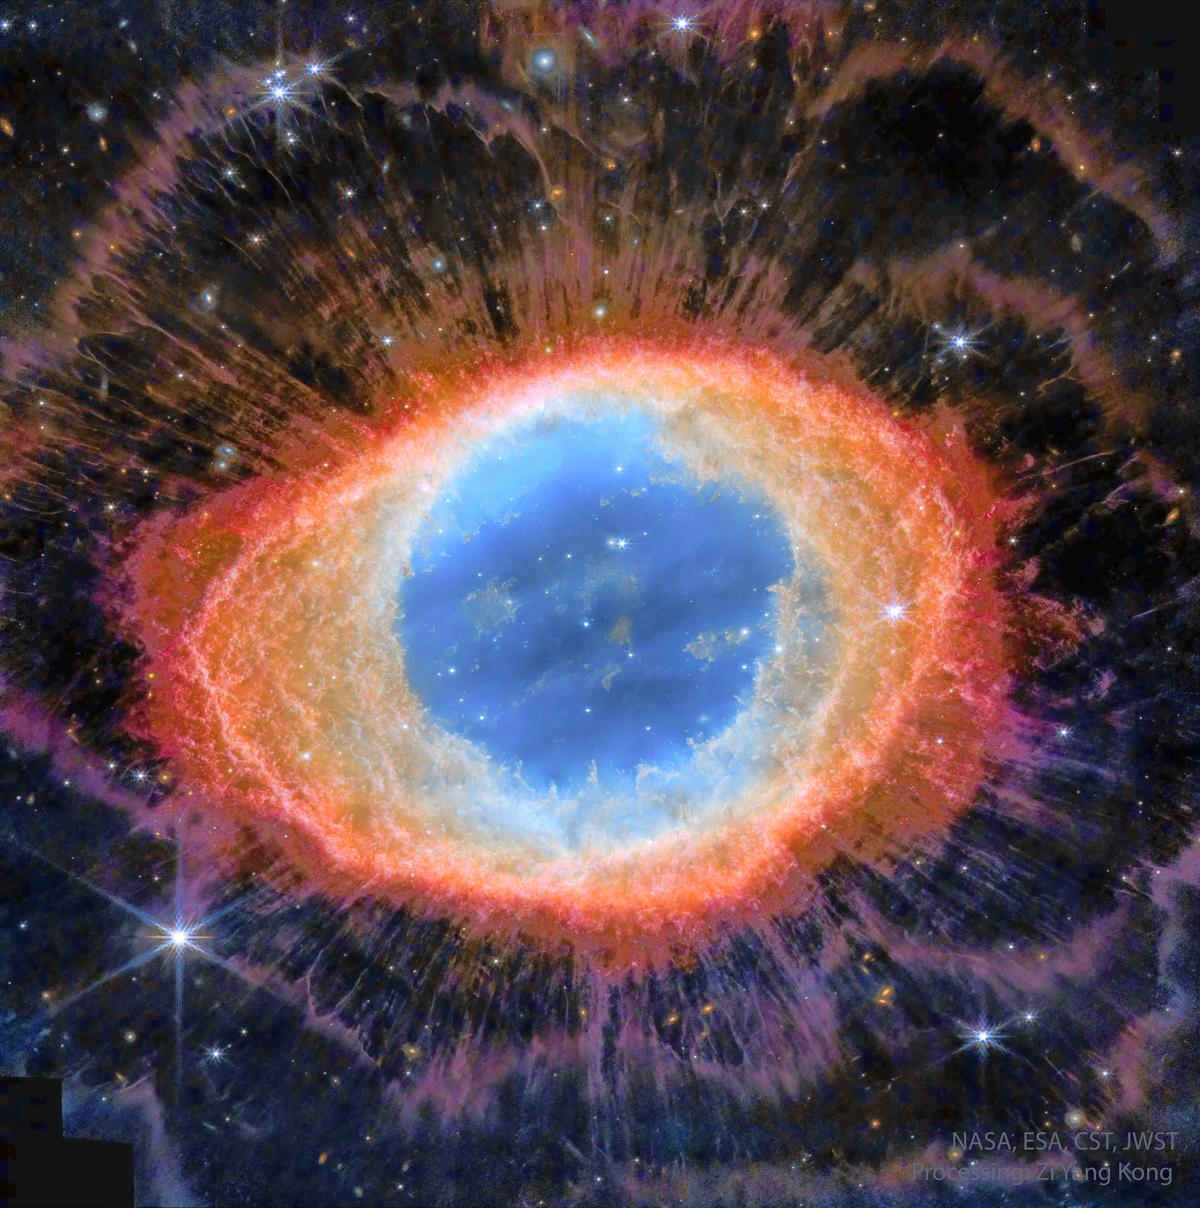
\includegraphics[width=0.85\textwidth]{img/ring_nebula_big.jpg}
\caption{Der Ringnebel M57 (JWST/Hubble): Ein kosmischer Torus. Die Natur formt toroidale Strukturen auf allen Skalen. Credit: NASA, ESA, CSA, JWST, HST; Processing: Zi Yang Kong.}
\end{figure}
Das Universum ist ein statischer, vierdimensionaler \textbf{Torsionskristall}. Die Raumzeit ist nicht das glatte, kontinuierliche Gebilde, das die Allgemeine Relativitätstheorie beschreibt. Auf der Sub-Planck-Skala besitzt sie eine diskrete, kristalline Struktur --- und das fundamentale geometrische Element dieser Struktur ist der \textbf{Torus}.

\section{Warum gerade der Torus?}

Unter allen geometrischen Formen ist der Torus einzigartig qualifiziert, die Architektur der Raumzeit zu tragen:

Er verbindet alle vier Dimensionen konsistent. Während die drei Raumdimensionen durch Tetraeder in dichtester Kugelpackung die lokale 3D-Kristallstruktur bilden, entsteht der Torus durch die vierte Dimension, die \enquote{aufgerollt} ist. Die Torsion --- die Windungen und Verdrillungen dieser Kristallstruktur --- ist das, was die Physik hervorbringt.

Der Torus ermöglicht die pentagonale Symmetriebrechung durch den goldenen Schnitt~$\varphi$. Er erzeugt natürlicherweise die Sub-Planck-Skala mit der Windungszahl $f = 7500 = 30000/4$. Diese Zahl $f = 2^2 \times 3 \times 5^4$ besitzt~36 Teiler und ist damit hochsymmetrisch --- ideal für die Resonanzstrukturen, die Teilchen hervorbringen.

\begin{figure}[ht]
\centering
\begin{tikzpicture}[scale=0.85]
  % Torus cross-section schematic
  % Outer circle (toroidal direction)
  \draw[thick, blue!40!black] (0,0) ellipse (3.5 and 1.2);
  % Inner tube cross-sections
  \draw[thick, blue!60!black, fill=blue!5] (-3.5,0) ellipse (0.6 and 0.9);
  \draw[thick, blue!60!black, fill=blue!5] (3.5,0) ellipse (0.6 and 0.9);
  % Top and bottom arcs (tube surface)
  \draw[thick, blue!50!black] (-3.5,0.9) arc (90:-90:0.15 and 0.9)
    [out=0,in=180] to (3.5,-0.9);
  \draw[thick, blue!50!black] (-3.5,-0.9) [out=0,in=180] to (3.5,-0.9);
  \draw[thick, blue!50!black] (-3.5,0.9) [out=0,in=180] to (3.5,0.9);

  % Labels: R and r
  \draw[<->, thick, red!60!black] (0,-0.15) -- (3.5,-0.15)
    node[midway, below, font=\small] {$R$};
  \draw[<->, thick, green!50!black] (3.5,0) -- (3.5,0.9)
    node[midway, right, font=\small] {$r$};

  % Energy flow arrows (toroidal)
  \foreach \a in {-2.5,-1.0,0.5,2.0} {
    \draw[-{Stealth[length=2.5mm]}, thick, orange!70!black]
      (\a,1.05) -- (\a+0.7,1.05);
  }
  \node[font=\footnotesize, orange!70!black] at (0,1.6) {Energiefluss (toroidal)};

  % Annotations right side
  \node[font=\small, text=blue!60!black, align=left] at (6.5,1.0) {Windungszahl};
  \node[font=\small, text=blue!60!black, align=left] at (6.5,0.5) {$f = 7500$};
  \node[font=\small, text=green!60!black, align=left] at (6.5,-0.3) {$\xi = 4/30000$};
  \node[font=\small, text=red!60!black, align=left] at (6.5,-0.9) {$D_f = 3 - \xi$};
  \node[font=\small, text=red!60!black, align=left] at (6.5,-1.4) {$\approx 2{,}9999$};

  % Center energy glow
  \shade[ball color=yellow!40!orange, opacity=0.3] (0,0) circle (0.8);
  \node[font=\footnotesize, text=orange!80!black] at (0,-1.8) {Vakuumenergie};
\end{tikzpicture}
\caption{Schematische Darstellung der Torus-Geometrie: Hauptradius~$R$, Röhrenradius~$r$, toroidaler Energiefluss und die Schlüsselparameter $f = 7500$, $\xi = 4/30000$, $D_f \approx 2{,}9999$.}
\label{fig:torus_schema}
\end{figure}

\section{Unendlich und begrenzt --- ohne Singularität}

Die entscheidende topologische Eigenschaft des Torus löst gleich mehrere der hartnäckigsten Probleme der Physik.

Der Torus hat \emph{endliches Volumen}, aber \emph{keine Ränder}. Man kann auf seiner Oberfläche unendlich weit wandern, ohne je an eine Grenze zu stoßen. Die Oberfläche ist geschlossen --- aber die Topologie allein schließt Singularitäten nicht aus. Entscheidend ist die Kombination der kompakten Topologie mit der \emph{Mediator-Masse~$m_T$} des Torsionsfeldes, die als natürlicher Regulator wirkt und den Kollaps zu Punktsingularitäten verhindert.

Die Konsequenzen dieser Kombination sind dramatisch:

Für \textbf{Schwarze Löcher} bedeutet das: Keine Punktsingularität. Stattdessen stabile Vakuumkerne, sogenannte T0-Knoten, die die toroidale Struktur stabilisieren. Der Kollaps zu einem Punkt unendlicher Dichte --- das Schreckgespenst der Allgemeinen Relativitätstheorie --- findet nicht statt. Die Mediator-Masse~$m_T$ des Torsionsfeldes wirkt wie eine natürliche Bremse.

Für den \textbf{Urknall} bedeutet das: Kein singulärer Anfangspunkt. Das Universum ist statisch und ewig. Es gab keinen Moment der Schöpfung im physikalischen Sinne --- das Universum \emph{ist}, als zeitlose Geometrie.

Für die \textbf{Feldtheorie} bedeutet das: Propagatoren divergieren nie. Die natürliche Regularisierung, die der Torus liefert, macht die aufwendigen Renormierungstechniken der Standard-QFT überflüssig. Die Unendlichkeiten, die Generationen von Physikern gequält haben, existieren schlicht nicht --- sie waren Artefakte einer falschen Annahme über die Topologie der Raumzeit.

Die Singularitätentheoreme von Penrose und Hawking --- die beweisen, dass Singularitäten in der ART \emph{unvermeidlich} sind --- werden damit aufgelöst. Die Theoreme gelten weiterhin, aber ihre Voraussetzungen (insbesondere die Energiebedingungen in nicht-kompakter Raumzeit) sind in T0 modifiziert: Die Mediator-Masse~$m_T$ ändert die effektive Energiebedingung nahe des Kollaps, während die kompakte Topologie die globale Struktur regularisiert.

Eine Analogie mag helfen: Die Oberfläche der Erde ist endlich, aber ohne Rand. Man fällt nie \enquote{vom Rand der Welt}. Ebenso ist das Universum im T0-Bild endlich im Volumen, aber ohne Grenzen --- und man trifft nie auf eine Singularität.

\section{Selbstähnlichkeit über alle Skalen}

Der Torus ist nicht nur auf der Sub-Planck-Skala relevant. Die toroidale Struktur wiederholt sich \emph{selbstähnlich} --- fraktal --- auf jeder Längenskala:

Von der Sub-Planck-Skala ($t_0 = \lP / 7500$) über Atomkerne und Atome, über Planeten und Sterne, über Galaxien bis zum gesamten Universum. Auf jeder Skala dieselbe grundlegende Geometrie, dieselbe Torsion, dieselben Resonanzen --- nur in verschiedenen Größenordnungen.

Das ist der tiefere Grund, warum~$\xsi$ universell ist: Der Parameter~$\xsi = 4/30000$ kodiert die Torsionsspannung auf \emph{jeder} Skala. Die Planck-Skala, die elektroschwache Skala, die QCD-Skala --- alles sind Resonanzen derselben Torusgeometrie.

\begin{kerngedanke}
Der Torus ist nicht ein geometrisches Modell unter vielen. Er ist das \emph{einzige} geometrische Objekt, das gleichzeitig endlich, randlos, singularitätsfrei und selbstähnlich ist --- und das alle vier Dimensionen konsistent verbindet. Die Physik wählt ihn nicht aus ästhetischen Gründen, sondern aus Notwendigkeit.
\end{kerngedanke}
